% The contents of this file is 
% Copyright (c) 2009-  Charles R. Severance, All Righs Reserved

\chapter{Visualizing data}

So far we have been learning the Python language and then 
learning how to use Python, the network, and databases 
to manipulate data.

In this chapter, we take a look at three 
complete applications that bring all of these things together
to manage and visualize data.  You  might use these applications 
as sample code to help get you started in solving a
real-world problem.

Each of the applications is a ZIP file that you can download
and extract onto your computer and execute.

\section{Building a Google map from geocoded data}
\index{Google!map}
\index{Visualization!map}

In this project, we are using the Google geocoding API
to clean up some user-entered geographic locations of 
university names and then placing the data on a Google
map.  

\beforefig
\centerline{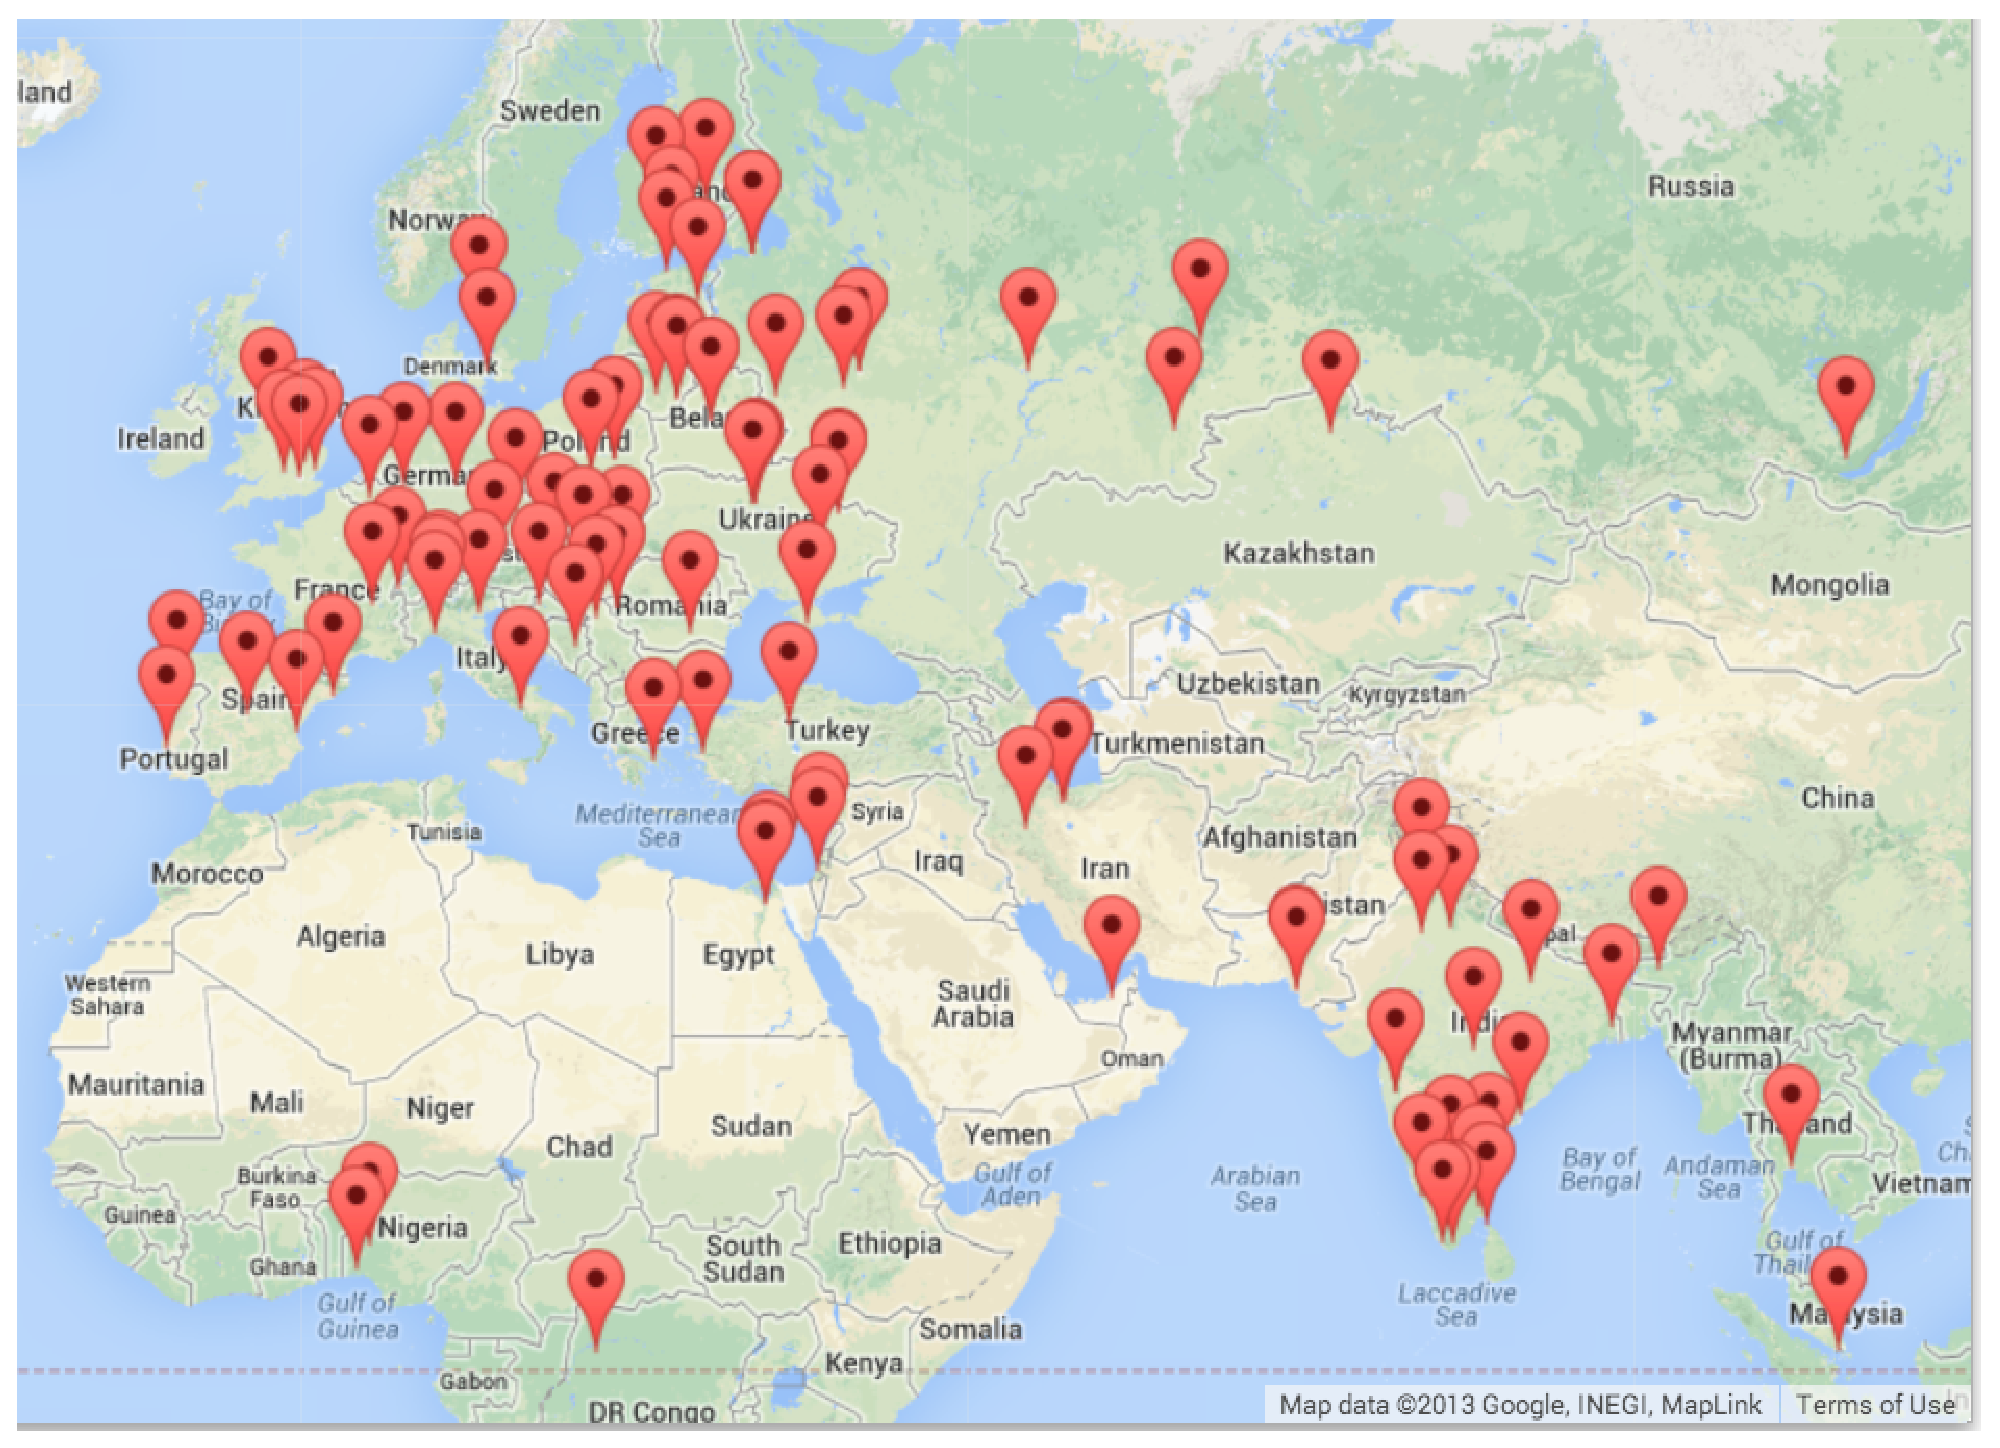
\includegraphics[height=2.25in]{figs2/google-map.eps}}
\afterfig

To get started, download the application from:

\url{www.py4inf.com/code/geodata.zip}

The first problem to solve is that the free Google geocoding
API is rate-limited to a certain number of requests per day.  If you have
a lot of data, you might need to stop and restart the lookup
process several times.  So we break the problem into two
phases.  

\index{cache}
In the first phase we take our input ``survey'' data in the file
{\bf where.data} and read it one line at a time, and retrieve the
geocoded information from Google and store it 
in a database {\bf geodata.sqlite}.
Before we use the geocoding API for each user-entered location, 
we simply check to see if we already have the data for that 
particular line of input.  The database is functioning as a 
local ``cache'' of our geocoding data to make sure we never ask 
Google for the same data twice.

You can restart the process at any time by removing the file
{\bf geodata.sqlite}.

Run the {\bf geoload.py} program.   This program will read the input
lines in {\bf where.data} and for each line check to see if it is already
in the database.  If we don't have the data for the location, it will
call the geocoding API to retrieve the data and store it in 
the database.

Here is a sample run after there is already some data in the 
database:

\beforeverb
\begin{verbatim}
Found in database  Northeastern University
Found in database  University of Hong Kong, ...
Found in database  Technion
Found in database  Viswakarma Institute, Pune, India
Found in database  UMD
Found in database  Tufts University

Resolving Monash University
Retrieving http://maps.googleapis.com/maps/api/
    geocode/json?sensor=false&address=Monash+University
Retrieved 2063 characters {    "results" : [  
{u'status': u'OK', u'results': ... }

Resolving Kokshetau Institute of Economics and Management
Retrieving http://maps.googleapis.com/maps/api/
    geocode/json?sensor=false&address=Kokshetau+Inst ...
Retrieved 1749 characters {    "results" : [  
{u'status': u'OK', u'results': ... }
...
\end{verbatim}
\afterverb
%
The first five locations are already in the database and so they 
are skipped.  The program scans to the point where it finds new
locations and starts retrieving them.

The {\bf geoload.py} program can be stopped at any time, and there is a counter 
that you can use to limit the number of calls to the geocoding
API for each run.  Given that the {\bf where.data} only has a few hundred
data items, you should not run into the daily rate limit, but if you 
had more data it might take several runs over several days to 
get your database to have all of the geocoded data for your input.

Once you have some data loaded into {\bf geodata.sqlite}, you can 
visualize the data using the {\bf geodump.py} program.  This
program reads the database and writes the file {\bf where.js}
with the location, latitude, and longitude in the form of
executable JavaScript code.   

A run of the {\bf geodump.py} program is as follows:

\beforeverb
\begin{verbatim}
Northeastern University, ... Boston, MA 02115, USA 42.3396998 -71.08975
Bradley University, 1501 ... Peoria, IL 61625, USA 40.6963857 -89.6160811
...
Technion, Viazman 87, Kesalsaba, 32000, Israel 32.7775 35.0216667
Monash University Clayton ... VIC 3800, Australia -37.9152113 145.134682
Kokshetau, Kazakhstan 53.2833333 69.3833333
...
12 records written to where.js
Open where.html to view the data in a browser
\end{verbatim}
\afterverb
%
The file {\bf where.html} consists of HTML and JavaScript to visualize 
a Google map.  It reads the most recent data in {\bf where.js} to get 
the data to be visualized.  Here is the format of the {\bf where.js} file:

\beforeverb
\begin{verbatim}
myData = [
[42.3396998,-71.08975, 'Northeastern Uni ... Boston, MA 02115'],
[40.6963857,-89.6160811, 'Bradley University, ... Peoria, IL 61625, USA'],
[32.7775,35.0216667, 'Technion, Viazman 87, Kesalsaba, 32000, Israel'],
   ...
];
\end{verbatim}
\afterverb
%
This is a JavaScript variable that contains a list of lists.  
The syntax for JavaScript list constants is very similar to 
Python, so the syntax should be familiar to you.

Simply open {\bf where.html} in a browser to see the locations.  You 
can hover over each map pin to find the location that the 
geocoding API returned for the user-entered input.  If you 
cannot see any data when you open the {\bf where.html} file, you might 
want to check the JavaScript or developer console for your browser.

\section{Visualizing networks and interconnections}
\index{Google!page rank}
\index{Visualization!networks}
\index{Visualization!page rank}

In this application, we will perform some of the functions of a search
engine.   We will first spider a small subset of the web and run
a simplified version of the Google page rank algorithm to
determine which pages are most highly connected, and then visualize
the page rank and connectivity of our small corner of the web.
We will use the D3 JavaScript visualization library 
\url{http://d3js.org/} to produce the visualization output.

You can download and extract this application from:

\url{www.py4inf.com/code/pagerank.zip}

\beforefig
\centerline{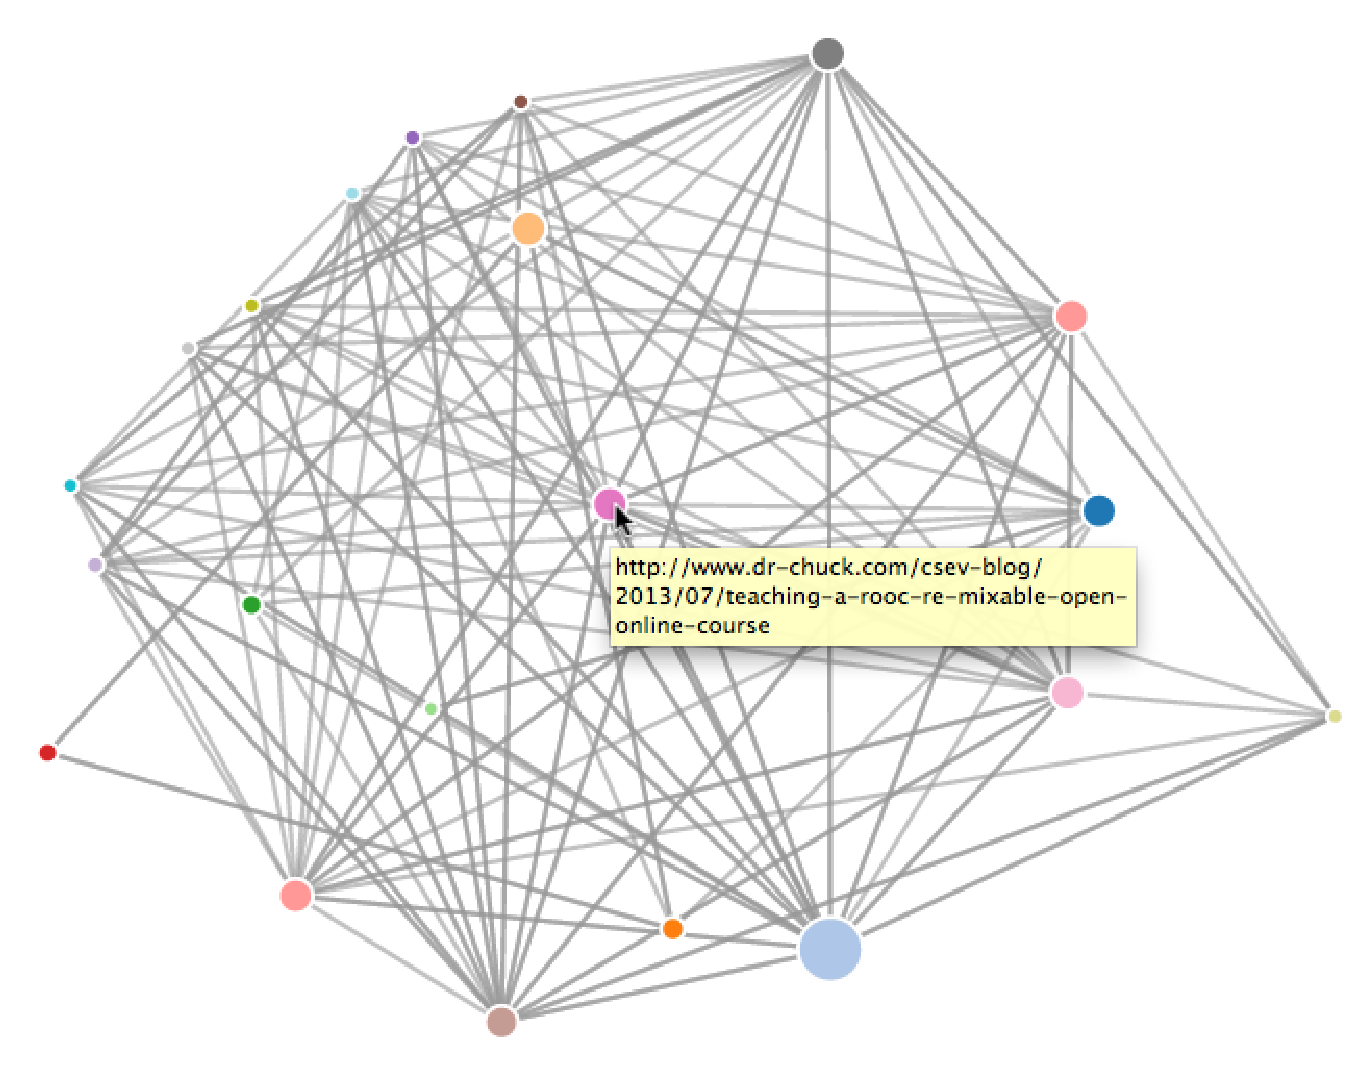
\includegraphics[height=2.25in]{figs2/pagerank.eps}}
\afterfig

The first program ({\bf spider.py}) program crawls a web 
site and pulls a series of pages into the
database ({\bf spider.sqlite}), recording the links between pages.
You can restart the process at any time by removing the 
{\bf spider.sqlite} file and rerunning {\bf spider.py}.

\beforeverb
\begin{verbatim}
Enter web url or enter: http://www.dr-chuck.com/
['http://www.dr-chuck.com']
How many pages:2
1 http://www.dr-chuck.com/ 12
2 http://www.dr-chuck.com/csev-blog/ 57
How many pages:
\end{verbatim}
\afterverb
%
In this sample run, we told it to crawl a website and retrieve two 
pages.  If you restart the program and tell it to crawl more
pages, it will not re-crawl any pages already in the database.  Upon 
restart it goes to a random non-crawled page and starts there.  So 
each successive run of {\bf spider.py} is additive.

\beforeverb
\begin{verbatim}
Enter web url or enter: http://www.dr-chuck.com/
['http://www.dr-chuck.com']
How many pages:3
3 http://www.dr-chuck.com/csev-blog 57
4 http://www.dr-chuck.com/dr-chuck/resume/speaking.htm 1
5 http://www.dr-chuck.com/dr-chuck/resume/index.htm 13
How many pages:
\end{verbatim}
\afterverb
%
You can have multiple starting points in the same database---within
the program, these are called ``webs''.   The spider
chooses randomly amongst all non-visited links across all
the webs as the next page to spider.

If you want to dump the contents of the {\bf spider.sqlite} file, you can 
run {\bf spdump.py} as follows:

\beforeverb
\begin{verbatim}
(5, None, 1.0, 3, u'http://www.dr-chuck.com/csev-blog')
(3, None, 1.0, 4, u'http://www.dr-chuck.com/dr-chuck/resume/speaking.htm')
(1, None, 1.0, 2, u'http://www.dr-chuck.com/csev-blog/')
(1, None, 1.0, 5, u'http://www.dr-chuck.com/dr-chuck/resume/index.htm')
4 rows.
\end{verbatim}
\afterverb
%
This shows the number of incoming links, the old page rank, the new page
rank, the id of the page, and the url of the page.  The {\bf spdump.py} program
only shows pages that have at least one incoming link to them.

Once you have a few pages in the database, you can run page rank on the
pages using the {\bf sprank.py} program.  You simply tell it how many page
rank iterations to run.

\beforeverb
\begin{verbatim}
How many iterations:2
1 0.546848992536
2 0.226714939664
[(1, 0.559), (2, 0.659), (3, 0.985), (4, 2.135), (5, 0.659)]
\end{verbatim}
\afterverb
%
You can dump the database again to see that page rank has been updated:

\beforeverb
\begin{verbatim}
(5, 1.0, 0.985, 3, u'http://www.dr-chuck.com/csev-blog')
(3, 1.0, 2.135, 4, u'http://www.dr-chuck.com/dr-chuck/resume/speaking.htm')
(1, 1.0, 0.659, 2, u'http://www.dr-chuck.com/csev-blog/')
(1, 1.0, 0.659, 5, u'http://www.dr-chuck.com/dr-chuck/resume/index.htm')
4 rows.
\end{verbatim}
\afterverb
%
You can run {\bf sprank.py} as many times as you like and it will simply refine
the page rank each time you run it.  You can even run {\bf sprank.py} a few times
and then go spider a few more pages sith {\bf spider.py} and then run {\bf sprank.py}
to reconverge the page rank values.  A search engine usually runs both the crawling and 
ranking programs all the time.

If you want to restart the page rank calculations without respidering the 
web pages, you can use {\bf spreset.py} and then restart {\bf sprank.py}.

\beforeverb
\begin{verbatim}
How many iterations:50
1 0.546848992536
2 0.226714939664
3 0.0659516187242
4 0.0244199333
5 0.0102096489546
6 0.00610244329379
...
42 0.000109076928206
43 9.91987599002e-05
44 9.02151706798e-05
45 8.20451504471e-05
46 7.46150183837e-05
47 6.7857770908e-05
48 6.17124694224e-05
49 5.61236959327e-05
50 5.10410499467e-05
[(512, 0.0296), (1, 12.79), (2, 28.93), (3, 6.808), (4, 13.46)]
\end{verbatim}
\afterverb
%
For each iteration of the page rank algorithm it prints the average
change in page rank per page.   The network initially is quite
unbalanced and so the individual page rank values change wildly between
iterations. But in a few short iterations, the page rank converges.  You
should run {\bf prank.py} long enough that the page rank values converge.

If you want to visualize the current top pages in terms of page rank,
run {\bf spjson.py} to read the database and write the data for the 
most highly linked pages in JSON format to be viewed in a
web browser.

\beforeverb
\begin{verbatim}
Creating JSON output on spider.json...
How many nodes? 30
Open force.html in a browser to view the visualization
\end{verbatim}
\afterverb
%
You can view this data by opening the file {\bf force.html} in your web browser.  
This shows an automatic layout of the nodes and links.  You can click and 
drag any node and you can also double-click on a node to find the URL
that is represented by the node.

If you rerun the other utilities, rerun {\bf spjson.py} and
press refresh in the browser to get the new data from {\bf spider.json}.

\section{Visualizing mail data}

Up to this point in the book, you have become quite familiar with our 
{\bf mbox-short.txt} and {\bf mbox.txt} data files.   Now it is time to take
our analysis of email data to the next level.  

In the real world, sometimes you have to pull down mail data from servers.
That might take quite some time and the data might be inconsistent, 
error-filled, and need a lot of cleanup or adjustment.  In this section, we
work with an application that is the most complex so far and pull down nearly a 
gigabyte of data and visualize it.

\beforefig
\centerline{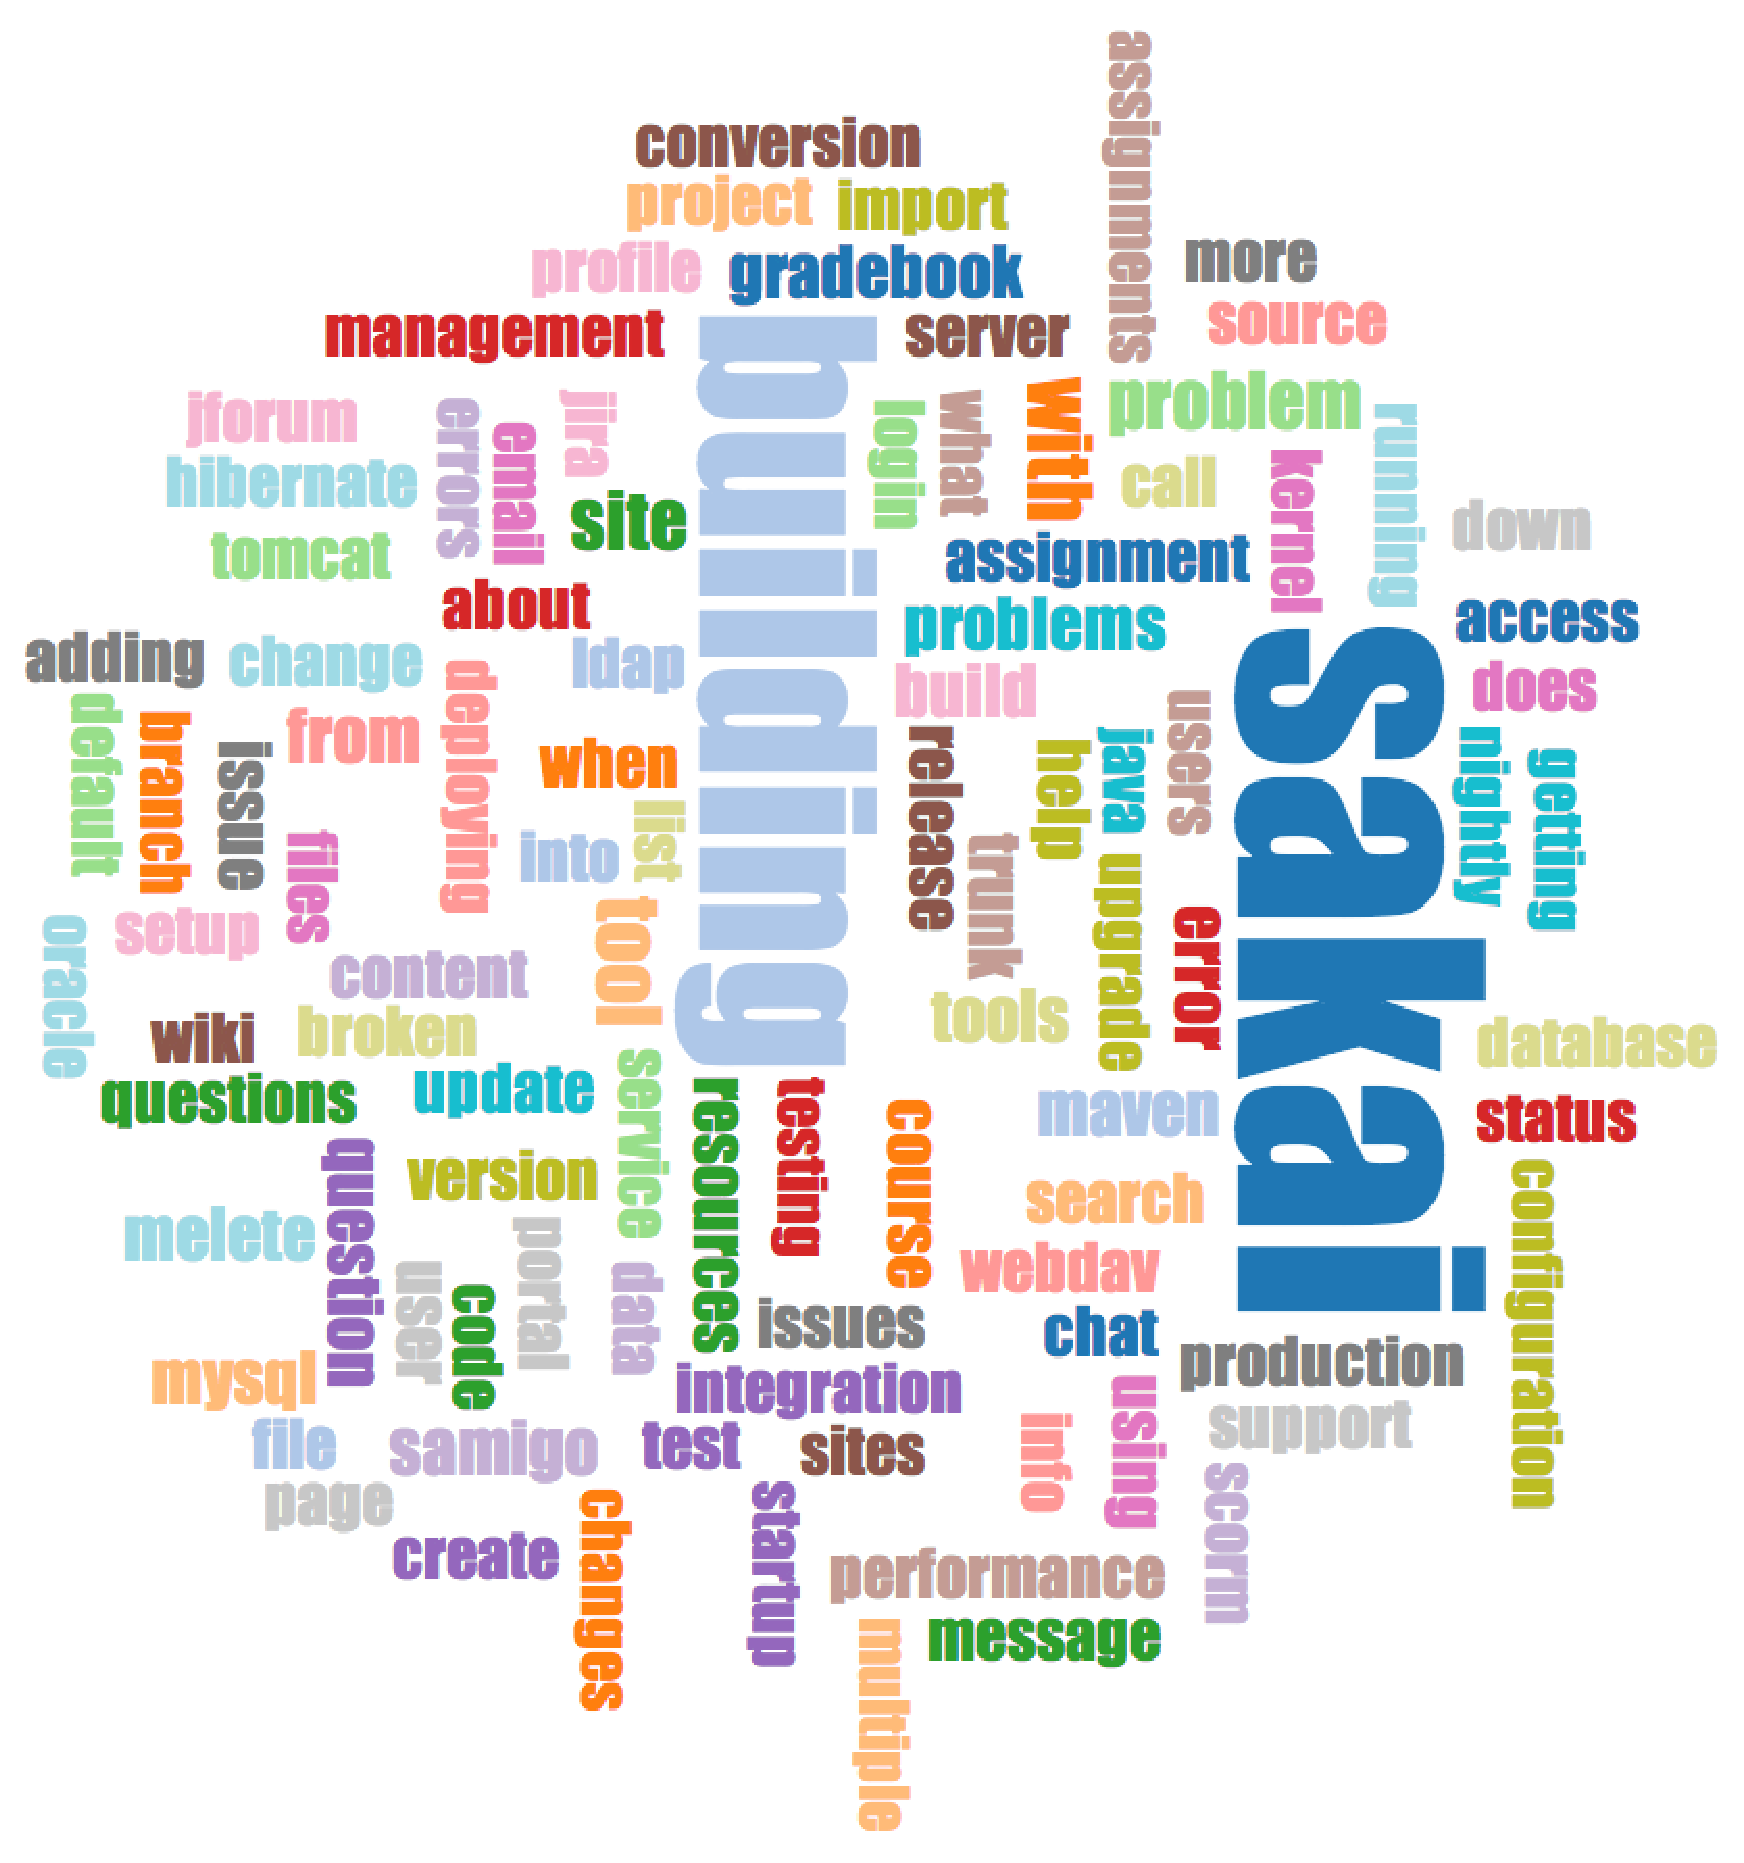
\includegraphics[height=2.50in]{figs2/wordcloud.eps}}
\afterfig

You can download this application from:

\url{www.py4inf.com/code/gmane.zip}

We will be using data from a free email list archiving service called 
\url{www.gmane.org}.  This service is very popular with open source
projects because it provides a nice searchable archive of their 
email activity.  They also have a very liberal policy regarding accessing 
their data through their API.  They have no rate limits, but ask that you 
don't overload their service and take only the data you need.  You can read
gmane's terms and conditions at this page:

\url{http://gmane.org/export.php}

{\em It is very important that you make use of the gmane.org data
responsibly by adding delays to your access of their services and spreading
long-running jobs over a longer period of time.  Do not abuse this free service
and ruin it for the rest of us.}

When the Sakai email data was spidered using this software, it produced nearly 
a Gigabyte of data and took a number of runs on several days.
The file {\bf README.txt} in the above ZIP may have instructions as to how
you can download a pre-spidered copy of the {\bf content.sqlite} file for 
a majority of the Sakai email corpus so you don't have to spider for 
five days just to run the programs.  If you download the pre-spidered
content, you should still run the spidering process to catch up with 
more recent messages.

The first step is to spider the gmane repository.  The base URL 
is hard-coded in the {\bf gmane.py} and is hard-coded to the Sakai
developer list.  You can spider another repository by changing that
base url.   Make sure to delete the {\bf content.sqlite} file if you 
switch the base url.  

The {\bf gmane.py} file operates as a responsible caching spider in 
that it runs slowly and retrieves one mail message per second so 
as to avoid getting throttled by gmane.   It stores all of
its data in a database and can be interrupted and restarted 
as often as needed.   It may take many hours to pull all the data
down.  So you may need to restart several times.

Here is a run of {\bf gmane.py} retrieving the last five messages of the
Sakai developer list:

\beforeverb
\begin{verbatim}
How many messages:10
http://download.gmane.org/gmane.comp.cms.sakai.devel/51410/51411 9460
    nealcaidin@sakaifoundation.org 2013-04-05 re: [building ...
http://download.gmane.org/gmane.comp.cms.sakai.devel/51411/51412 3379
    samuelgutierrezjimenez@gmail.com 2013-04-06 re: [building ...
http://download.gmane.org/gmane.comp.cms.sakai.devel/51412/51413 9903
    da1@vt.edu 2013-04-05 [building sakai] melete 2.9 oracle ...
http://download.gmane.org/gmane.comp.cms.sakai.devel/51413/51414 349265
    m.shedid@elraed-it.com 2013-04-07 [building sakai] ...
http://download.gmane.org/gmane.comp.cms.sakai.devel/51414/51415 3481
    samuelgutierrezjimenez@gmail.com 2013-04-07 re: ...
http://download.gmane.org/gmane.comp.cms.sakai.devel/51415/51416 0

Does not start with From 
\end{verbatim}
\afterverb
%
The program scans {\bf content.sqlite} from one up to the first message number not
already spidered and starts spidering at that message.  It continues spidering
until it has spidered the desired number of messages or it reaches a page
that does not appear to be a properly formatted message.

Sometimes \url{gmane.org} is missing a message.  Perhaps administrators can delete messages
or perhaps they get lost.   If your spider stops, and it seems it has hit
a missing message, go into the SQLite Manager and add a row with the missing id leaving
all the other fields blank and restart {\bf gmane.py}.   This will unstick the 
spidering process and allow it to continue.  These empty messages will be ignored in the next
phase of the process.

One nice thing is that once you have spidered all of the messages and have them in 
{\bf content.sqlite}, you can run {\bf gmane.py} again to get new messages as 
they are sent to the list.  

The {\bf content.sqlite} data is pretty raw, with an inefficient data model, 
and not compressed.
This is intentional as it allows you to look at {\bf content.sqlite}
in the SQLite Manager to debug problems with the spidering process.
It would be a bad idea to run any queries against this database, as they 
would be quite slow.

The second process is to run the program {\bf gmodel.py}.  This program reads the raw 
data from {\bf content.sqlite} and produces a cleaned-up and well-modeled version of the 
data in the file {\bf index.sqlite}.  This file will be much smaller (often 10X
smaller) than {\bf content.sqlite} because it also compresses the header and body text.

Each time {\bf gmodel.py} runs it deletes and rebuilds {\bf index.sqlite}, allowing
you to adjust its parameters and edit the mapping tables in {\bf content.sqlite} to tweak the 
data cleaning process. This is a sample run of {\bf gmodel.py}.  It prints a line out each time
250 mail messages are processed so you can see some progress happening, as this program may
run for a while processing nearly a Gigabyte of mail data.

\beforeverb
\begin{verbatim}
Loaded allsenders 1588 and mapping 28 dns mapping 1
1 2005-12-08T23:34:30-06:00 ggolden22@mac.com
251 2005-12-22T10:03:20-08:00 tpamsler@ucdavis.edu
501 2006-01-12T11:17:34-05:00 lance@indiana.edu
751 2006-01-24T11:13:28-08:00 vrajgopalan@ucmerced.edu
...
\end{verbatim}
\afterverb
%

The {\bf gmodel.py} program handles a number of data cleaning tasks.

Domain names are truncated to two levels for .com, .org, .edu, and .net.
Other domain names are truncated to three levels.  So si.umich.edu becomes
umich.edu and caret.cam.ac.uk becomes cam.ac.uk.   Email addresses are also
forced to lower case, and some of the @gmane.org address like the following

\beforeverb
\begin{verbatim}
   arwhyte-63aXycvo3TyHXe+LvDLADg@public.gmane.org
\end{verbatim}
\afterverb
%
are converted to the real address whenever there is a matching real email
address elsewhere in the message corpus.

In the {\bf content.sqlite} database there are two tables that allow
you to map both domain names and individual email addresses that change over 
the lifetime of the email list.  For example, Steve Githens used the following
email addresses as he changed jobs over the life of the Sakai developer list:

\beforeverb
\begin{verbatim}
s-githens@northwestern.edu
sgithens@cam.ac.uk
swgithen@mtu.edu
\end{verbatim}
\afterverb
%
We can add two entries to the Mapping table in {\bf content.sqlite} so 
{\bf gmodel.py} will map all three to one address:

\beforeverb
\begin{verbatim}
s-githens@northwestern.edu ->  swgithen@mtu.edu
sgithens@cam.ac.uk -> swgithen@mtu.edu
\end{verbatim}
\afterverb
%
You can also make similar entries in the DNSMapping table if there are multiple
DNS names you want mapped to a single DNS.  The following mapping was added to the Sakai data:

\beforeverb
\begin{verbatim}
iupui.edu -> indiana.edu
\end{verbatim}
\afterverb
%
so all the accounts from the various Indiana University campuses are tracked together.

You can rerun the {\bf gmodel.py} over and over as you look at the data, and add mappings
to make the data cleaner and cleaner.   When you are done, you will have a nicely
indexed version of the email in {\bf index.sqlite}.   This is the file to use to do data
analysis.   With this file, data analysis will be really quick.

The first, simplest data analysis is to determine "who sent the most mail?" and "which 
organization sent the most mail"?  This is done using {\bf gbasic.py}:

\beforeverb
\begin{verbatim}
How many to dump? 5
Loaded messages= 51330 subjects= 25033 senders= 1584

Top 5 Email list participants
steve.swinsburg@gmail.com 2657
azeckoski@unicon.net 1742
ieb@tfd.co.uk 1591
csev@umich.edu 1304
david.horwitz@uct.ac.za 1184

Top 5 Email list organizations
gmail.com 7339
umich.edu 6243
uct.ac.za 2451
indiana.edu 2258
unicon.net 2055
\end{verbatim}
\afterverb
%
Note how much more quickly {\bf gbasic.py} runs compared to {\bf gmane.py}
or even {\bf gmodel.py}. They are all working on the same data, but 
{\bf gbasic.py} is using the compressed and normalized data in 
{\bf index.sqlite}.  If you have a lot of data to manage, a multistep
process like the one in this application may take a little longer to develop,
but will save you a lot of time when you really start to explore
and visualize your data.

You can produce a simple visualization of the word frequency in the subject lines
in the file {\bf gword.py}:

\beforeverb
\begin{verbatim}
Range of counts: 33229 129
Output written to gword.js
\end{verbatim}
\afterverb
%

This produces the file {\bf gword.js} which you can visualize using
{\bf gword.htm} to produce a word cloud similar to the one at the beginning 
of this section.

A second visualization is produced  by {\bf gline.py}.  It computes email 
participation by organizations over time.

\beforeverb
\begin{verbatim}
Loaded messages= 51330 subjects= 25033 senders= 1584
Top 10 Oranizations
['gmail.com', 'umich.edu', 'uct.ac.za', 'indiana.edu', 
'unicon.net', 'tfd.co.uk', 'berkeley.edu', 'longsight.com', 
'stanford.edu', 'ox.ac.uk']
Output written to gline.js
\end{verbatim}
\afterverb
%
Its output is written to {\bf gline.js} which is visualized using {\bf gline.htm}.

\beforefig
\centerline{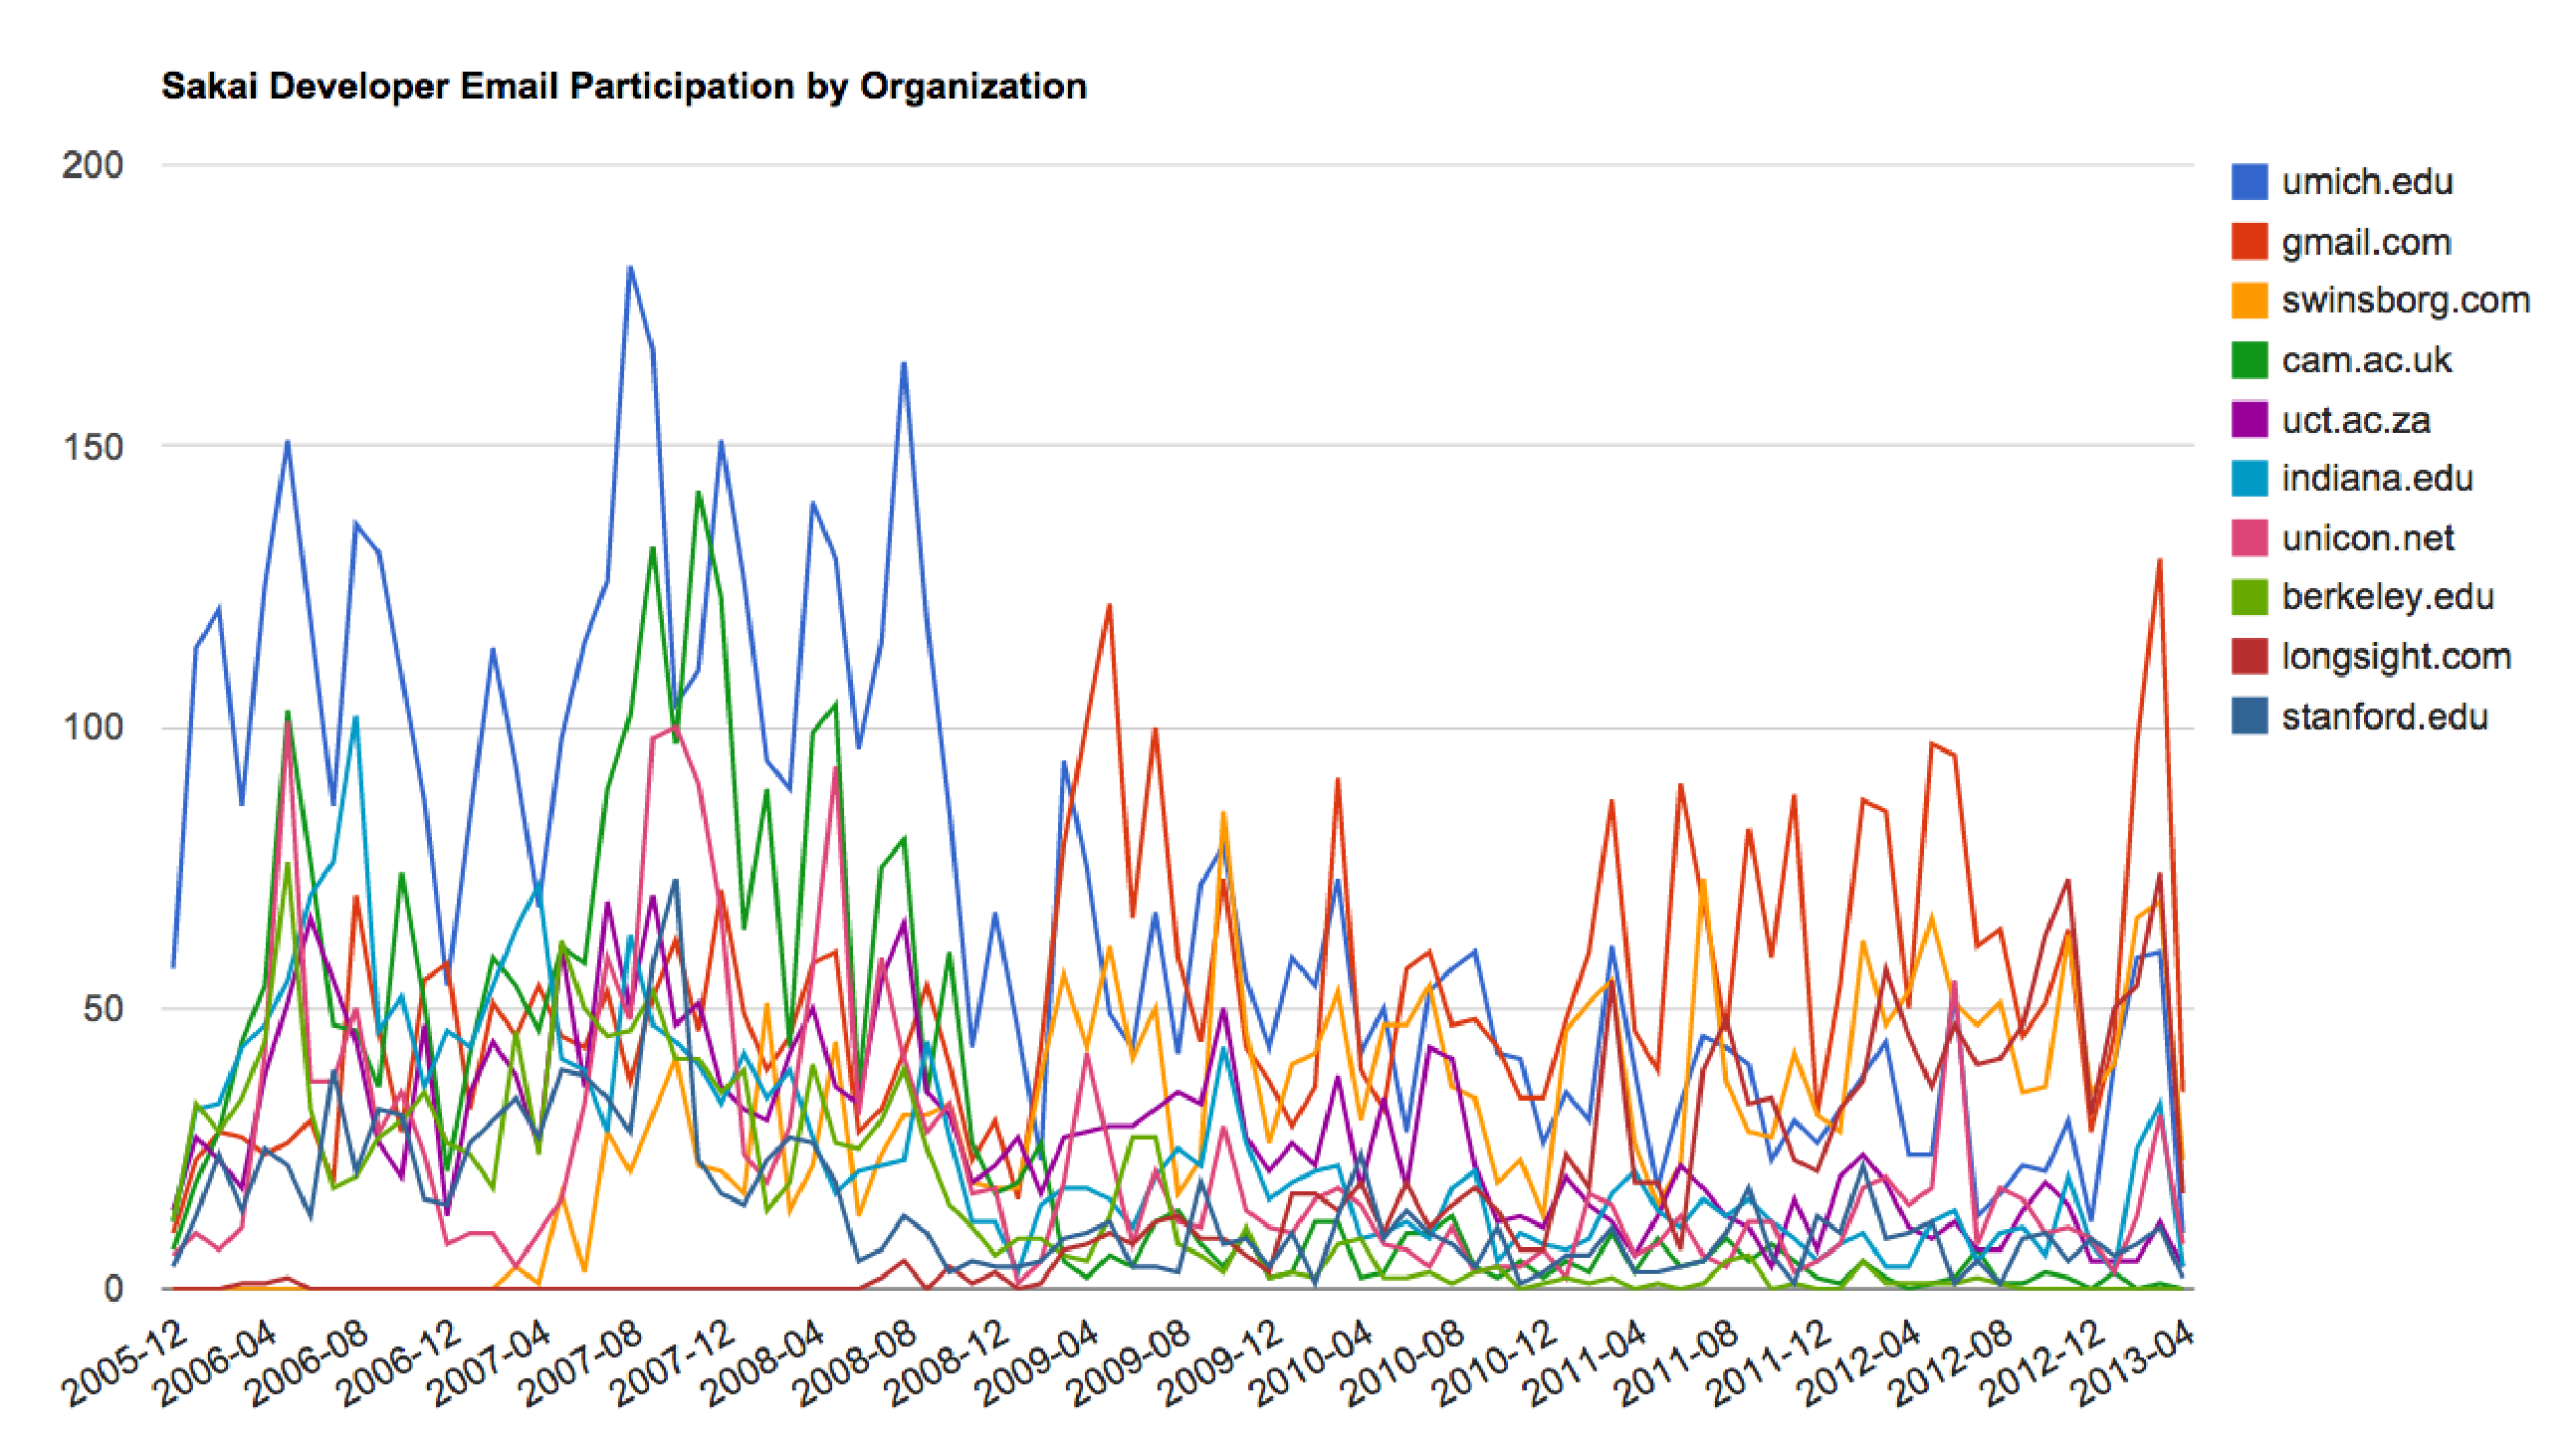
\includegraphics[height=2.50in]{figs2/mailorg.eps}}
\afterfig

This is a relatively complex and sophisticated application and 
has features to do some real data retrieval, cleaning, and visualization.
